\section{The Wolf-Goat-Cabbage Problem}

  \subsection{Question 1}

    Below is a graph representing the relationships between all possible states
    in the Wolf-Goat-Cabbage Problem. In this graphic:

    \begin{itemize}
      \item \textcolor{gray}{\textbf{Grey}} edges represent a movement of the
      boat with no animals.
      \item \textcolor{green}{\textbf{Green}} edges represent a movement with
      the cabbage on the boat.
      \item \textcolor{cyan}{\textbf{Blue}} edges represent a movement with the
      goat on the boat.
      \item \textcolor{red}{\textbf{Red}} edges represent a movement with the
      wolf on the boat.
    \end{itemize}
    \bigskip
    All edges are considered bidirectional (since the activities can be done in
    reverse).
    \bigskip
    


\newarray\states
\readarray{states}{1111 & 1110 & 1101 & 1100 & 1011 & 1010 & 1001 & 1000 & 0111 & 0110 & 0101 & 0100 & 0011 & 0010 & 0001 & 0000}


\noindent\makebox[\textwidth]{%
    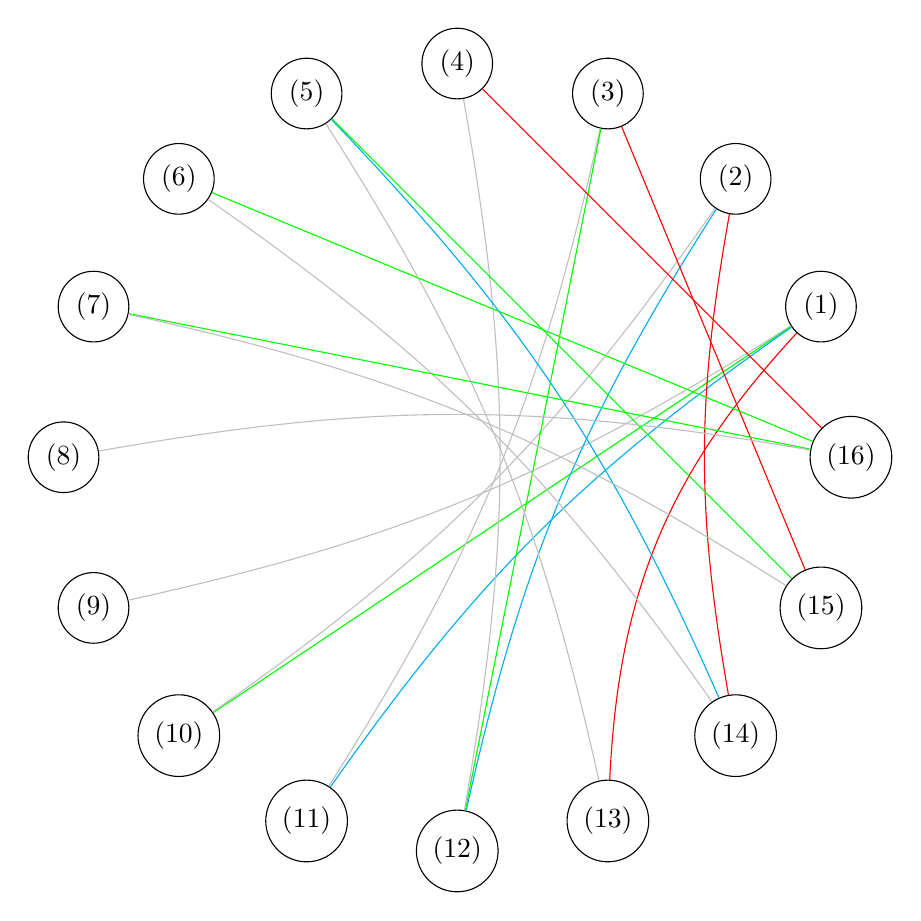
\begin{tikzpicture}[block/.style={circle,thick}]

        \foreach \a in {1,...,16}{
            \draw (\a*360/16: 5cm) node[shape=circle,draw=black](\a){\states(\a)};
        }

    \fill[fill=red] (1);
    \draw ->(1);
    \draw (1) to[bend left=10] (9)  [draw=lightgray];
    \draw (1) to (10) [draw=green];
    \draw (1) to[bend right=10] (11) [draw=cyan];
    \draw (1) to[bend right=20] (13) [draw=red];

    \draw (2) to[bend left=10] (10) [draw=lightgray];
    \draw (2) to[bend right=10] (12) [draw=cyan];
    \draw (2) to[bend right=10] (14) [draw=red];

    \draw (3) to[bend left=10] (11) [draw=lightgray];
    \draw (3) to (12) [draw=green];
    \draw (3) to (15) [draw=red];

    \draw (4) to[bend left=10] (12) [draw=lightgray];
    \draw (4) to (16) [draw=red];

    \draw (5) to[bend left=10] (13) [draw=lightgray];
    \draw (5) to[bend left=10] (14) [draw=cyan];
    \draw (5) to (15) [draw=green];

    \draw (6) to[bend left=10] (14) [draw=lightgray];
    \draw (6) to (16) [draw=green];

    \draw (7) to (16) [draw=green];
    \draw (7) to[bend left=10] (15) [draw=lightgray];

    \draw (8) to[bend left=10] (16) [draw=lightgray];



    \end{tikzpicture}
}


  \pagebreak
  \subsection{Question 2}

  Below is a tree representation of actions that may be taken to convert all
actors being on one bank to another. The children are ordered left-to-right
\textbf{B}(oat), \textbf{W}(olf), \textbf{G}(oat), \textbf{C}(abbage), meaning
that a movement of the boat with no animals will always appear as the most left
child (if such a move is possible).
\\\\
Further, the error states (ie. all leaves that
are not the goal state), are written $A \rightarrow B$, which reads as ``A
consumes B''.

    \bigskip

    \noindent\makebox[\textwidth]{%
\Tree [.1111
  [.0111
    \textit{$G \rightarrow C$/$W \rightarrow G$}
  ]
  [.0011
    \textit{$G \rightarrow C$}
  ]
  [.0101 [.1101
    [.0001
      [.1001
        \textit{$W \rightarrow G$}
      ]
      [.1011 [.0010
        [. 1010 [. \textbf{0000} ]]
        [. 1110
          [. 0100
            [. 1100
              \textit{$G \rightarrow C$}
            ]
          ]
        ]
      ]]
    ]
    [.0100
      [. 1110
        [.0110
          \textit{$W \rightarrow G$}
        ]
        [.0010
          [.1010
            \textbf{0000}
          ]
        ]
      ]
      [.1101
        [.0001
          [.1001
            \textit{$W \rightarrow G$}
          ]
          [.1011
            [.0010
              [. 1010
                \textbf{0000}
              ]
              [. 1110
                [.0110
                  \textit{$W \rightarrow G$}
                ]
              ]
            ]
          ]
        ]
      ]
    ]
  ]]
  [.0110
    \textit{$W \rightarrow G$}
  ]
]
}


  \subsection{Question 3}

    \bigskip

    $$1111 \rightarrow 0101 \rightarrow 1101 \rightarrow 0001 \rightarrow 1011
    \rightarrow 0010 \rightarrow 1010 \rightarrow 0000$$
